\documentclass[norsk]{beamer}				% frames
%\documentclass[notes, norsk]{beamer}		% frames + notes
%\documentclass[notes=only]{beamer}	% notes
\usepackage[utf8]{inputenc}		% for UTF8 characters
\usepackage{babel}		% manages typographical rules for English
\usepackage{csquotes}			% quotes that support babel
\usepackage{graphicx} 			% include graphics
\usepackage{verbatim} 			% include files with special characters
\usepackage{tabularx}			% fancy tables
\usepackage{booktabs}			% lines in tables
\usepackage{mathbbol}			% bold math symbols
\usepackage{float}				% fix object
\usepackage{color}				% colors
\usepackage{array} 				% for column alignment
\usepackage{listings}			% listings of code
\usepackage{hyperref}			% cross-reference
\usepackage{amsmath}			% various math symbols
\usepackage{physics}			% Dirac notation and matrices
\usepackage{amssymb}			% more math symbols
\usepackage{comment}			% in-line comments
\usepackage{makecell}			% new line in cell
\usepackage{subfig}				% sub figures
\usepackage{empheq}				% beautiful equation boxes
\usepackage{multirow}			% multirow in table
\usepackage{multicol}			% multicolumn in table
\usepackage{varwidth}			% rotate text in table
\usepackage{arydshln}   		% dashed lines in table
\usepackage{framed}
\usepackage{xargs} 
\usepackage{copyrightbox}		% copyright of images
\usepackage{mathpazo}  			% consistent nice math font 
\usepackage{mathtools}			% more math symbols
\usepackage{appendixnumberbeamer}	% appendix slides (backup slides)
\usepackage{pgfpages}			% separate note slides

% biblatex
\usepackage[backend=bibtex,
			%sorting=none,
			style=nature
]{biblatex}
\addbibresource{refs.bib}

% footnote position in slides
\usepackage[absolute,
			overlay
]{textpos}

% beamer presentation tool for Linux (display frames and notes separately)
%\usepackage[duration=35, 
%			lastminutes=10
%]{pdfpcnotes} 

% colors
\definecolor{maincolor}{RGB}{28, 39, 131}			% to be used in titles, progression wheel and references
\definecolor{empheqbackground}{RGB}{153, 153, 255}	% to be used as equation and quote background

\captionsetup[figure]{labelfont={color=maincolor}}
\captionsetup[table]{labelfont={color=maincolor}}

%empheq equation color box
\newlength\mytemplen
\newsavebox\mytempbox

\makeatletter
\newcommand\mybluebox{%
	\@ifnextchar[%]
	{\@mybluebox}%
	{\@mybluebox[0pt]}}

\def\@mybluebox[#1]{%
	\@ifnextchar[%]
	{\@@mybluebox[#1]}%
	{\@@mybluebox[#1][0pt]}}

\def\@@mybluebox[#1][#2]#3{
	\sbox\mytempbox{#3}%
	\mytemplen\ht\mytempbox
	\advance\mytemplen #1\relax
	\ht\mytempbox\mytemplen
	\mytemplen\dp\mytempbox
	\advance\mytemplen #2\relax
	\dp\mytempbox\mytemplen
	\colorbox{empheqbackground}{\hspace{1em}\usebox{\mytempbox}\hspace{1em}}}

% double quotes
\newcommand*\openquote{\makebox(40,-5){\scalebox{5}{``}}}
\newcommand*\closequote{\makebox(25,-22){\scalebox{5}{''}}}
\colorlet{shadecolor}{empheqbackground}
\makeatletter
\newif\if@right
\def\shadequote{\@righttrue\shadequote@i}
\def\shadequote@i{\begin{snugshade}\begin{quote}\openquote}
		\def\endshadequote{%
			\if@right\hfill\fi\closequote\end{quote}\end{snugshade}}
\@namedef{shadequote*}{\@rightfalse\shadequote@i}
\@namedef{endshadequote*}{\endshadequote}
\makeatother

% Beamer style
 \setlength{\TPHorizModule}{10mm}
\setlength{\TPVertModule}{\TPHorizModule}
\textblockorigin{1mm}{1mm} % start everything near the top-left corner
\setlength{\parindent}{0pt}

\setbeamertemplate{itemize items}{\color{maincolor}$\blacktriangleright$}  % triangular bullet points
\setbeamertemplate{bibliography item}{\insertbiblabel}                      % for reference slide
\setbeameroption{show notes on second screen=right}                         % where to display notes
\addtobeamertemplate{footnote}{}{\vspace{10ex}}								% footnote spacing
\mathtoolsset{showonlyrefs}													% ignore unused references
\usefonttheme{serif}														% serif font
\renewcommand*{\thefootnote}{\fnsymbol{footnote}}							% special characters as footnote symbols
\renewcommand*{\bibfont}{\tiny}												% reference fontsize tiny

\setbeamercolor{titlelike}{fg=black}
\setbeamercolor{block title}{fg=white}
\setbeamercolor{block title}{bg=black}
\setbeamercolor{block body}{bg=maincolor}

\setbeamerfont{itemize/enumerate body}{size=\scriptsize}
\setbeamerfont{itemize/enumerate subbody}{size=\scriptsize}
\setbeamerfont{itemize/enumerate subsubbody}{size=\scriptsize}


%%%%%%%%%%%%%%%%%%%%%%%%%%%%%%%%%%%%%%%%%%%%%%%%%%%%%%%%%%%%%%%%%%%%%%%%%%%%%%%%%%%%%%%%%%%%%%%%%%%%%%%%%%%%%%%%%%%%%
% FRONT FRAME
%%%%%%%%%%%%%%%%%%%%%%%%%%%%%%%%%%%%%%%%%%%%%%%%%%%%%%%%%%%%%%%%%%%%%%%%%%%%%%%%%%%%%%%%%%%%%%%%%%%%%%%%%%%%%%%%%%%%%
\newcommand{\frontframe}{
	\begin{frame}
		%\titlepage 
		\thispagestyle{empty}
		\begin{center}
			\Large{\textcolor{black}{\mtitle}}\\ \vspace{0.5cm}
			\includegraphics[scale=.3]{../images/UiO_Segl_pms485.eps} \\ \vspace{0.5cm}
			\large{\mauthor}\\ \vspace{0.3cm}
			\scriptsize{Universitet i Oslo} \\ \vspace{0.2cm}
			\scriptsize{\textit{\mmail}} \\ \vspace{0.5cm}
			\large{\today} \\ \vfill
		\end{center}
	\end{frame}
}

%%%%%%%%%%%%%%%%%%%%%%%%%%%%%%%%%%%%%%%%%%%%%%%%%%%%%%%%%%%%%%%%%%%%%%%%%%%%%%%%%%%%%%%%%%%%%%%%%%%%%%%%%%%%%%%%%%%%%
% ORDINARY FRAME
%%%%%%%%%%%%%%%%%%%%%%%%%%%%%%%%%%%%%%%%%%%%%%%%%%%%%%%%%%%%%%%%%%%%%%%%%%%%%%%%%%%%%%%%%%%%%%%%%%%%%%%%%%%%%%%%%%%%%
\newcommand{\mframe}[3]{
	\frame{
		% PROGRESSION WHEEL 
		\begin{textblock}{3}(0.5,8)
			\begin{tikzpicture}[x=1mm,y=1mm]
			\foreach \x in {1,2,...,\inserttotalframenumber} 
			\draw [gray!30,very thick] (\x/\inserttotalframenumber*360:3) -- (\x/\inserttotalframenumber*360:4);
			\foreach \x in {1,2,...,\insertframenumber}
			\draw[maincolor,very thick] (\x/\inserttotalframenumber*360:3) -- (\x/\inserttotalframenumber*360:4);
			\node at (0,0) [] {\tiny{\textbf{\textcolor{black}{\insertframenumber}}}};
			\end{tikzpicture}
		\end{textblock}
	
		% UIO LOGO
		\begin{textblock}{3}(4.2,8.3)
			\centering
			
\includegraphics[scale=.2]{../images/UiO_Segl_A_cmyk.eps}
		\end{textblock}
		\frametitle{\textcolor{maincolor}{#1}}
		\framesubtitle{#2}
		\vspace{-0.5cm}
		\scriptsize{#3}}
}

%%%%%%%%%%%%%%%%%%%%%%%%%%%%%%%%%%%%%%%%%%%%%%%%%%%%%%%%%%%%%%%%%%%%%%%%%%%%%%%%%%%%%%%%%%%%%%%%%%%%%%%%%%%%%%%%%%%%%
% TITLED FRAME
%%%%%%%%%%%%%%%%%%%%%%%%%%%%%%%%%%%%%%%%%%%%%%%%%%%%%%%%%%%%%%%%%%%%%%%%%%%%%%%%%%%%%%%%%%%%%%%%%%%%%%%%%%%%%%%%%%%%%
\newcommand{\titleframe}[1]{
	\mframe{}{}{
		\begin{center}
			{\Huge \textcolor{maincolor}{#1}}
		\end{center}
	}
}
% include definitions
\newcommand{\citet}[1]{\citeauthor{#1} \supercite{#1}}

%%%%%%%%%%%%%%%%%%%%%%%%%%%%%%%%%%%%%%%%%%%%%%%%%%%%%%%%%%%%%%%%%%%%%%%%%%%%%%%%%%%%%%%%%%%%%%%%%%%%%%%%%%%%%%%%%%%%%
% SPECIFY INFORMATION TO BE USED IN FRONT FRAME
%%%%%%%%%%%%%%%%%%%%%%%%%%%%%%%%%%%%%%%%%%%%%%%%%%%%%%%%%%%%%%%%%%%%%%%%%%%%%%%%%%%%%%%%%%%%%%%%%%%%%%%%%%%%%%%%%%%%%

\newcommand{\mtitle}{Maskinlæring}
\newcommand{\mauthor}{Even Marius Nordhagen}
\newcommand{\mmail}{evenmn@fys.uio.no}
\newcommand{\massignn}{.}

\begin{document}

\frontframe

\note{
	\begin{itemize}
		\item This is an example presentation about quantum mechanics
		\item The front frame is generated using \textit{frontframe}
		\item Note also that the notes can be turned on and off in the first line of this file
	\end{itemize}
}

\mframe{Oversikt}{}{
	\begin{itemize}
		\setlength\itemsep{1em}	% This line specifies the spacing between bullet points
		\item Motivasjon
		\item Teorien bak
		\item Implementasjon
		\item Dere skal implementere et nevralt nettverk
	\end{itemize}
}

\note{Dette er planen for dagen}

\titleframe{Motivasjon}

\mframe{Regresjon}{}{
	Regresjon er en enkel form for maskinlæring
	
	\begin{figure}
		\centering
		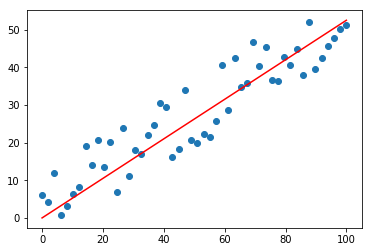
\includegraphics[width=6cm]{../images/regression.png}
	\end{figure}
}

\note{Konsept dere kanskje er kjente med}

\mframe{Bildeanalyse}{}{
	Kjenne igjen hva som er på et bilde og hvor objektene befinner seg
	\begin{figure}
		\centering
		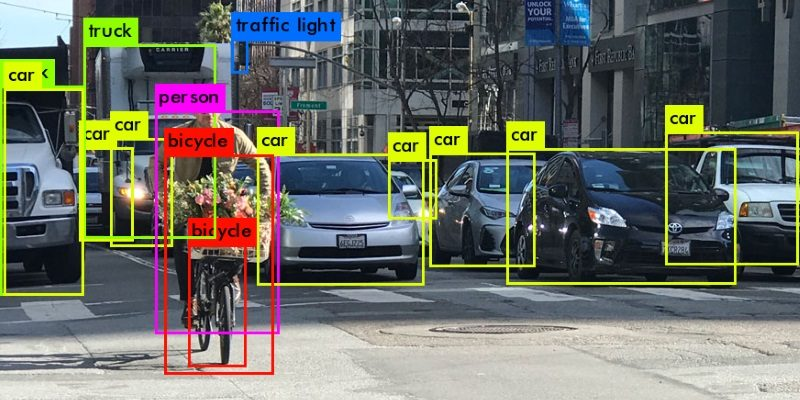
\includegraphics[width=10cm]{../images/image_recognition.jpg}
	\end{figure}
}

\note{kfkffk}

\mframe{Generative modeller}{}{
	\begin{figure}
		\centering
		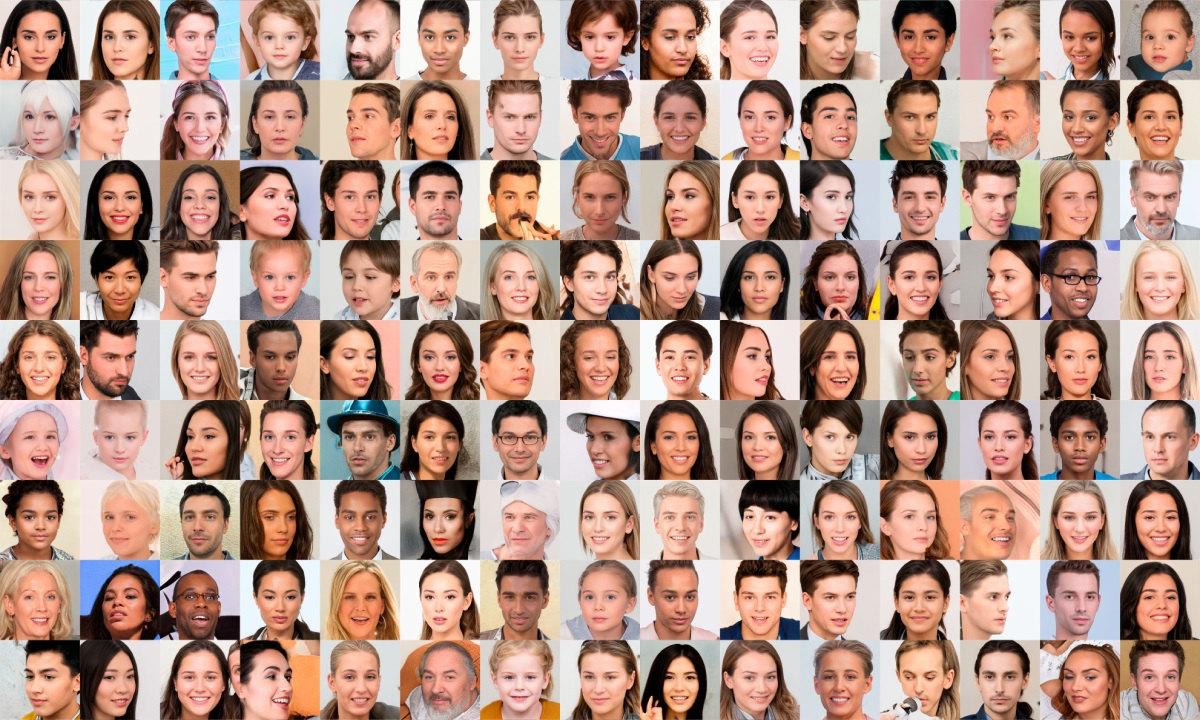
\includegraphics[width=10cm]{../images/aifaces_feat.jpg}
	\end{figure}
}

\mframe{Andre eksempler}{}{
	\begin{itemize}
		\setlength\itemsep{1em}	% This line specifies the spacing between bullet points
		\item Stemmegjenkjenning
		\item Taktikkspill
		\item Autonom teknologi
	\end{itemize}
}

\titleframe{Nevrale nettverk}

\mframe{Hva er et nevralt nettverk?}{}{
	\begin{itemize}
		\setlength\itemsep{2em}
		\item<1-> Inspirert av biologi og hjerneforskning
		\item<2-> Fleksible funksjoner $\rightarrow$ mange parametere
		\item<3-> Feedforward nettverk kan representere enhver funksjon
	\end{itemize}
	\note <1>{Basert på studier av hvordan hjernen lærer}
	\note <2->{Feedforward er det viktigste nevrale nettverket, og det som ofte brukes til å illustrere et nevralt nettverk. Ved å justere parameterne i et feedforward nettverk, kan man tilpasse enhver kontinuerlig funksjon.} 
}

\mframe{Nevralt nettverk: Feedforward}{Fase: Fremover}{
	\begin{figure}
		\centering
		\begin{overprint}[9cm]
			\onslide<1>\begin{tikzpicture}

% Define outputs
\node[] (center) {};
\node[input, above=0.3em of center] (y1) {};
\node[input, below=0.3em of center] (y2) {};

% Draw lines from output nodes
\node[right of=y1] (righty1) {};
\node[right of=y2] (righty2) {};
\path[draw,->] (y1) -- (righty1);
\path[draw,->] (y2) -- (righty2);

% Hidden nodes L
\node[input,left=5em of center] (aL3) {};
\node[input,above of=aL3] (aL2) {};
\node[input,above of=aL2] (aL1) {};
\node[input,below of=aL3] (aL4) {};
\node[input,below of=aL4] (aL5) {};

% Hidden nodes 1
\node[input,left=15em of center] (a13) {};
\node[input,above of=a13] (a12) {};
\node[input,above of=a12] (a11) {};
\node[input,below of=a13] (a14) {};
\node[input,below of=a14] (a15) {};

% Draw lines from hidden nodes
\path[draw,->] (aL1) -- (y1);
\path[draw,->] (aL2) -- (y1);
\path[draw,->] (aL3) -- (y1);
\path[draw,->] (aL4) -- (y1);
\path[draw,->] (aL5) -- (y1);

\path[draw,->] (aL1) -- (y2);
\path[draw,->] (aL2) -- (y2);
\path[draw,->] (aL3) -- (y2);
\path[draw,->] (aL4) -- (y2);
\path[draw,->] (aL5) -- (y2);

% Define place left of left
\node[input,left=5em of a13, fill=red] (x2) {};
\node[input,above of=x2, fill=red] (x1) {};
\node[input,below of=x2, fill=red] (x3) {};

% Draw lines from input nodes
\path[draw,->] (x1) -- (a11);
\path[draw,->] (x1) -- (a12);
\path[draw,->] (x1) -- (a13);
\path[draw,->] (x1) -- (a14);
\path[draw,->] (x1) -- (a15);

\path[draw,->] (x2) -- (a11);
\path[draw,->] (x2) -- (a12);
\path[draw,->] (x2) -- (a13);
\path[draw,->] (x2) -- (a14);
\path[draw,->] (x2) -- (a15);

\path[draw,->] (x3) -- (a11);
\path[draw,->] (x3) -- (a12);
\path[draw,->] (x3) -- (a13);
\path[draw,->] (x3) -- (a14);
\path[draw,->] (x3) -- (a15);

% Draw lines from first hidden layer
\path[draw,->] (a11) -- (aL1);
\path[draw,->] (a11) -- (aL2);
\path[draw,->] (a11) -- (aL3);
\path[draw,->] (a11) -- (aL4);
\path[draw,->] (a11) -- (aL5);

\path[draw,->] (a12) -- (aL1);
\path[draw,->] (a12) -- (aL2);
\path[draw,->] (a12) -- (aL3);
\path[draw,->] (a12) -- (aL4);
\path[draw,->] (a12) -- (aL5);

\path[draw,->] (a13) -- (aL1);
\path[draw,->] (a13) -- (aL2);
\path[draw,->] (a13) -- (aL3);
\path[draw,->] (a13) -- (aL4);
\path[draw,->] (a13) -- (aL5);

\path[draw,->] (a14) -- (aL1);
\path[draw,->] (a14) -- (aL2);
\path[draw,->] (a14) -- (aL3);
\path[draw,->] (a14) -- (aL4);
\path[draw,->] (a14) -- (aL5);

\path[draw,->] (a15) -- (aL1);
\path[draw,->] (a15) -- (aL2);
\path[draw,->] (a15) -- (aL3);
\path[draw,->] (a15) -- (aL4);
\path[draw,->] (a15) -- (aL5);


% Draw lines towards input nodes
\node[left of=x1] (leftx1) {};
\node[left of=x2] (leftx2) {};
\node[left of=x3] (leftx3) {};
\path[draw,->] (leftx1) -- (x1);
\path[draw,->] (leftx2) -- (x2);
\path[draw,->] (leftx3) -- (x3); 

\end{tikzpicture}
			\onslide<2>\begin{tikzpicture}

% Define outputs
\node[] (center) {};
\node[input, above=0.3em of center] (y1) {};
\node[input, below=0.3em of center] (y2) {};

% Draw lines from output nodes
\node[right of=y1] (righty1) {};
\node[right of=y2] (righty2) {};
\path[draw,->] (y1) -- (righty1);
\path[draw,->] (y2) -- (righty2);

% Hidden nodes L
\node[input,left=5em of center] (aL3) {};
\node[input,above of=aL3] (aL2) {};
\node[input,above of=aL2] (aL1) {};
\node[input,below of=aL3] (aL4) {};
\node[input,below of=aL4] (aL5) {};

% Hidden nodes 1
\node[input,left=15em of center, fill=red] (a13) {};
\node[input,above of=a13, fill=red] (a12) {};
\node[input,above of=a12, fill=red] (a11) {};
\node[input,below of=a13, fill=red] (a14) {};
\node[input,below of=a14, fill=red] (a15) {};

% Draw lines from hidden nodes
\path[draw,->] (aL1) -- (y1);
\path[draw,->] (aL2) -- (y1);
\path[draw,->] (aL3) -- (y1);
\path[draw,->] (aL4) -- (y1);
\path[draw,->] (aL5) -- (y1);

\path[draw,->] (aL1) -- (y2);
\path[draw,->] (aL2) -- (y2);
\path[draw,->] (aL3) -- (y2);
\path[draw,->] (aL4) -- (y2);
\path[draw,->] (aL5) -- (y2);

% Define place left of left
\node[input,left=5em of a13] (x2) {};
\node[input,above of=x2] (x1) {};
\node[input,below of=x2] (x3) {};

% Draw lines from input nodes
\path[draw,->] (x1) -- (a11);
\path[draw,->] (x1) -- (a12);
\path[draw,->] (x1) -- (a13);
\path[draw,->] (x1) -- (a14);
\path[draw,->] (x1) -- (a15);

\path[draw,->] (x2) -- (a11);
\path[draw,->] (x2) -- (a12);
\path[draw,->] (x2) -- (a13);
\path[draw,->] (x2) -- (a14);
\path[draw,->] (x2) -- (a15);

\path[draw,->] (x3) -- (a11);
\path[draw,->] (x3) -- (a12);
\path[draw,->] (x3) -- (a13);
\path[draw,->] (x3) -- (a14);
\path[draw,->] (x3) -- (a15);

% Draw lines from first hidden layer
\path[draw,->] (a11) -- (aL1);
\path[draw,->] (a11) -- (aL2);
\path[draw,->] (a11) -- (aL3);
\path[draw,->] (a11) -- (aL4);
\path[draw,->] (a11) -- (aL5);

\path[draw,->] (a12) -- (aL1);
\path[draw,->] (a12) -- (aL2);
\path[draw,->] (a12) -- (aL3);
\path[draw,->] (a12) -- (aL4);
\path[draw,->] (a12) -- (aL5);

\path[draw,->] (a13) -- (aL1);
\path[draw,->] (a13) -- (aL2);
\path[draw,->] (a13) -- (aL3);
\path[draw,->] (a13) -- (aL4);
\path[draw,->] (a13) -- (aL5);

\path[draw,->] (a14) -- (aL1);
\path[draw,->] (a14) -- (aL2);
\path[draw,->] (a14) -- (aL3);
\path[draw,->] (a14) -- (aL4);
\path[draw,->] (a14) -- (aL5);

\path[draw,->] (a15) -- (aL1);
\path[draw,->] (a15) -- (aL2);
\path[draw,->] (a15) -- (aL3);
\path[draw,->] (a15) -- (aL4);
\path[draw,->] (a15) -- (aL5);


% Draw lines towards input nodes
\node[left of=x1] (leftx1) {};
\node[left of=x2] (leftx2) {};
\node[left of=x3] (leftx3) {};
\path[draw,->] (leftx1) -- (x1);
\path[draw,->] (leftx2) -- (x2);
\path[draw,->] (leftx3) -- (x3); 
\end{tikzpicture}
			\onslide<3>\begin{tikzpicture}

% Define outputs
\node[] (center) {};
\node[input, above=0.3em of center] (y1) {};
\node[input, below=0.3em of center] (y2) {};

% Draw lines from output nodes
\node[right of=y1] (righty1) {};
\node[right of=y2] (righty2) {};
\path[draw,->] (y1) -- (righty1);
\path[draw,->] (y2) -- (righty2);

% Hidden nodes L
\node[input,left=5em of center, fill=red] (aL3) {};
\node[input,above of=aL3, fill=red] (aL2) {};
\node[input,above of=aL2, fill=red] (aL1) {};
\node[input,below of=aL3, fill=red] (aL4) {};
\node[input,below of=aL4, fill=red] (aL5) {};

% Hidden nodes 1
\node[input,left=15em of center] (a13) {};
\node[input,above of=a13] (a12) {};
\node[input,above of=a12] (a11) {};
\node[input,below of=a13] (a14) {};
\node[input,below of=a14] (a15) {};

% Draw lines from hidden nodes
\path[draw,->] (aL1) -- (y1);
\path[draw,->] (aL2) -- (y1);
\path[draw,->] (aL3) -- (y1);
\path[draw,->] (aL4) -- (y1);
\path[draw,->] (aL5) -- (y1);

\path[draw,->] (aL1) -- (y2);
\path[draw,->] (aL2) -- (y2);
\path[draw,->] (aL3) -- (y2);
\path[draw,->] (aL4) -- (y2);
\path[draw,->] (aL5) -- (y2);

% Define place left of left
\node[input,left=5em of a13] (x2) {};
\node[input,above of=x2] (x1) {};
\node[input,below of=x2] (x3) {};

% Draw lines from input nodes
\path[draw,->] (x1) -- (a11);
\path[draw,->] (x1) -- (a12);
\path[draw,->] (x1) -- (a13);
\path[draw,->] (x1) -- (a14);
\path[draw,->] (x1) -- (a15);

\path[draw,->] (x2) -- (a11);
\path[draw,->] (x2) -- (a12);
\path[draw,->] (x2) -- (a13);
\path[draw,->] (x2) -- (a14);
\path[draw,->] (x2) -- (a15);

\path[draw,->] (x3) -- (a11);
\path[draw,->] (x3) -- (a12);
\path[draw,->] (x3) -- (a13);
\path[draw,->] (x3) -- (a14);
\path[draw,->] (x3) -- (a15);

% Draw lines from first hidden layer
\path[draw,->] (a11) -- (aL1);
\path[draw,->] (a11) -- (aL2);
\path[draw,->] (a11) -- (aL3);
\path[draw,->] (a11) -- (aL4);
\path[draw,->] (a11) -- (aL5);

\path[draw,->] (a12) -- (aL1);
\path[draw,->] (a12) -- (aL2);
\path[draw,->] (a12) -- (aL3);
\path[draw,->] (a12) -- (aL4);
\path[draw,->] (a12) -- (aL5);

\path[draw,->] (a13) -- (aL1);
\path[draw,->] (a13) -- (aL2);
\path[draw,->] (a13) -- (aL3);
\path[draw,->] (a13) -- (aL4);
\path[draw,->] (a13) -- (aL5);

\path[draw,->] (a14) -- (aL1);
\path[draw,->] (a14) -- (aL2);
\path[draw,->] (a14) -- (aL3);
\path[draw,->] (a14) -- (aL4);
\path[draw,->] (a14) -- (aL5);

\path[draw,->] (a15) -- (aL1);
\path[draw,->] (a15) -- (aL2);
\path[draw,->] (a15) -- (aL3);
\path[draw,->] (a15) -- (aL4);
\path[draw,->] (a15) -- (aL5);


% Draw lines towards input nodes
\node[left of=x1] (leftx1) {};
\node[left of=x2] (leftx2) {};
\node[left of=x3] (leftx3) {};
\path[draw,->] (leftx1) -- (x1);
\path[draw,->] (leftx2) -- (x2);
\path[draw,->] (leftx3) -- (x3); 
\end{tikzpicture}
			\onslide<4>\begin{tikzpicture}

% Define outputs
\node[] (center) {};
\node[input, above=0.3em of center, fill=red] (y1) {};
\node[input, below=0.3em of center, fill=red] (y2) {};

% Draw lines from output nodes
\node[right of=y1] (righty1) {};
\node[right of=y2] (righty2) {};
\path[draw,->, color=red] (y1) -- (righty1);
\path[draw,->, color=red] (y2) -- (righty2);

% Hidden nodes L
\node[input,left=5em of center] (aL3) {};
\node[input,above of=aL3] (aL2) {};
\node[input,above of=aL2] (aL1) {};
\node[input,below of=aL3] (aL4) {};
\node[input,below of=aL4] (aL5) {};

% Hidden nodes 1
\node[input,left=15em of center] (a13) {};
\node[input,above of=a13] (a12) {};
\node[input,above of=a12] (a11) {};
\node[input,below of=a13] (a14) {};
\node[input,below of=a14] (a15) {};

% Draw lines from hidden nodes
\path[draw,->] (aL1) -- (y1);
\path[draw,->] (aL2) -- (y1);
\path[draw,->] (aL3) -- (y1);
\path[draw,->] (aL4) -- (y1);
\path[draw,->] (aL5) -- (y1);

\path[draw,->] (aL1) -- (y2);
\path[draw,->] (aL2) -- (y2);
\path[draw,->] (aL3) -- (y2);
\path[draw,->] (aL4) -- (y2);
\path[draw,->] (aL5) -- (y2);

% Define place left of left
\node[input,left=5em of a13] (x2) {};
\node[input,above of=x2] (x1) {};
\node[input,below of=x2] (x3) {};

% Draw lines from input nodes
\path[draw,->] (x1) -- (a11);
\path[draw,->] (x1) -- (a12);
\path[draw,->] (x1) -- (a13);
\path[draw,->] (x1) -- (a14);
\path[draw,->] (x1) -- (a15);

\path[draw,->] (x2) -- (a11);
\path[draw,->] (x2) -- (a12);
\path[draw,->] (x2) -- (a13);
\path[draw,->] (x2) -- (a14);
\path[draw,->] (x2) -- (a15);

\path[draw,->] (x3) -- (a11);
\path[draw,->] (x3) -- (a12);
\path[draw,->] (x3) -- (a13);
\path[draw,->] (x3) -- (a14);
\path[draw,->] (x3) -- (a15);

% Draw lines from first hidden layer
\path[draw,->] (a11) -- (aL1);
\path[draw,->] (a11) -- (aL2);
\path[draw,->] (a11) -- (aL3);
\path[draw,->] (a11) -- (aL4);
\path[draw,->] (a11) -- (aL5);

\path[draw,->] (a12) -- (aL1);
\path[draw,->] (a12) -- (aL2);
\path[draw,->] (a12) -- (aL3);
\path[draw,->] (a12) -- (aL4);
\path[draw,->] (a12) -- (aL5);

\path[draw,->] (a13) -- (aL1);
\path[draw,->] (a13) -- (aL2);
\path[draw,->] (a13) -- (aL3);
\path[draw,->] (a13) -- (aL4);
\path[draw,->] (a13) -- (aL5);

\path[draw,->] (a14) -- (aL1);
\path[draw,->] (a14) -- (aL2);
\path[draw,->] (a14) -- (aL3);
\path[draw,->] (a14) -- (aL4);
\path[draw,->] (a14) -- (aL5);

\path[draw,->] (a15) -- (aL1);
\path[draw,->] (a15) -- (aL2);
\path[draw,->] (a15) -- (aL3);
\path[draw,->] (a15) -- (aL4);
\path[draw,->] (a15) -- (aL5);


% Draw lines towards input nodes
\node[left of=x1] (leftx1) {};
\node[left of=x2] (leftx2) {};
\node[left of=x3] (leftx3) {};
\path[draw,->] (leftx1) -- (x1);
\path[draw,->] (leftx2) -- (x2);
\path[draw,->] (leftx3) -- (x3); 

%\node[below=3em of y2] {$\tilde{\bs{y}}$};
\end{tikzpicture}
		\end{overprint}
	\end{figure}
	\note<1->{Dette nettverket tar inn en input med informasjon på venstre side. Denne informasjonen blir deretter matet fremover i nettverket, og er derfor kalt et feedforward nevralt nettverk. For at nettverket skal trenes opp, trenger vi targets som forteller hva vi forventer å få ut med noen gitte inputs. Man sammenligner deretter det nettverket gir ut med det man forventer. }
}

\mframe{Nevralt nettverk: Feedforward}{Aktiveringsfunksjon}{
	En aktiveringsfunksjon brukes for å \textit{aktivere} inputen til hvert lag. Rectified Linear Unit (ReLU) er en vanlig funksjon:
	\begin{figure}
		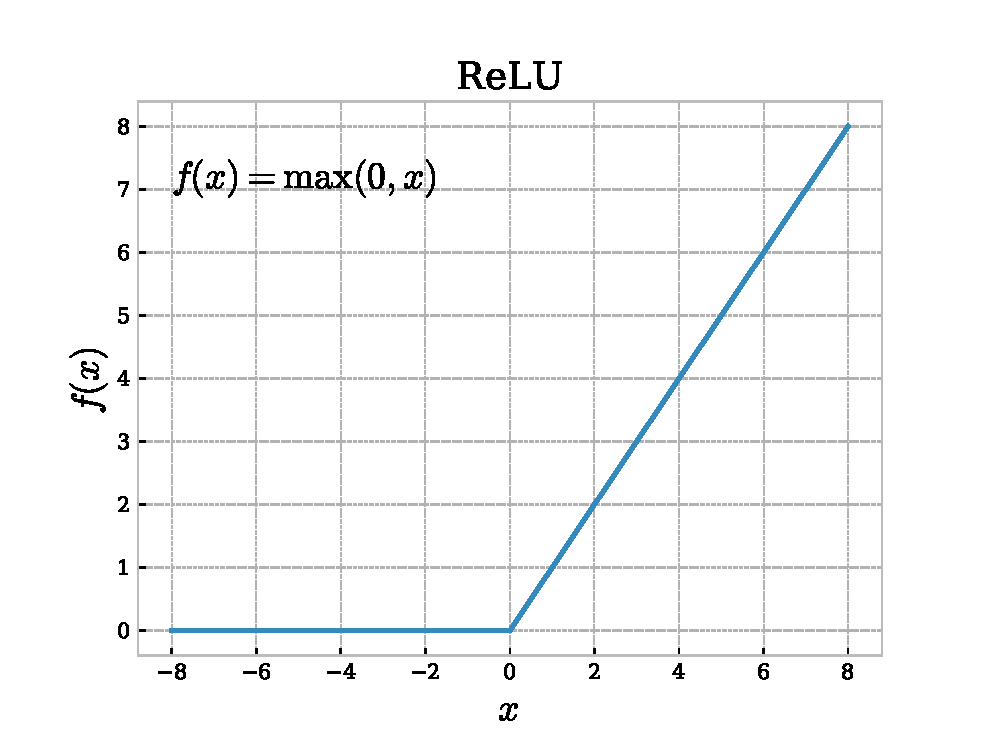
\includegraphics[scale=.3]{../images/ReLU.eps}
	\end{figure}
}

\mframe{Nevralt nettverk: Feedforward}{Feilestimat}{
	En mye brukt kostfunksjon er minste kvadraters metode: 
	\begin{equation}
	\mathcal{C} = \frac{1}{2}\left(\boldsymbol{y}-\tilde{\boldsymbol{y}}\right)^2
	\end{equation}
}
\note{Feilen defineres av en kostfunksjon. Det er mange typer kostfunksjoner.}

\mframe{Nevralt nettverk: Feedforward}{Fase: Bakover}{
	\begin{figure}
		\centering
		\begin{overprint}[9cm]
			\onslide<1>\begin{tikzpicture}

% Define outputs
\node[] (center) {};
\node[input, above=0.3em of center, fill=red] (y1) {};
\node[input, below=0.3em of center, fill=red] (y2) {};

% Draw lines from output nodes
\node[right of=y1] (righty1) {};
\node[right of=y2] (righty2) {};
\path[draw,->, color=red] (y1) -- (righty1);
\path[draw,->, color=red] (y2) -- (righty2);

% Hidden nodes L
\node[input,left=5em of center] (aL3) {};
\node[input,above of=aL3] (aL2) {};
\node[input,above of=aL2] (aL1) {};
\node[input,below of=aL3] (aL4) {};
\node[input,below of=aL4] (aL5) {};

% Hidden nodes 1
\node[input,left=15em of center] (a13) {};
\node[input,above of=a13] (a12) {};
\node[input,above of=a12] (a11) {};
\node[input,below of=a13] (a14) {};
\node[input,below of=a14] (a15) {};

% Draw lines from hidden nodes
\path[draw,->] (aL1) -- (y1);
\path[draw,->] (aL2) -- (y1);
\path[draw,->] (aL3) -- (y1);
\path[draw,->] (aL4) -- (y1);
\path[draw,->] (aL5) -- (y1);

\path[draw,->] (aL1) -- (y2);
\path[draw,->] (aL2) -- (y2);
\path[draw,->] (aL3) -- (y2);
\path[draw,->] (aL4) -- (y2);
\path[draw,->] (aL5) -- (y2);

% Define place left of left
\node[input,left=5em of a13] (x2) {};
\node[input,above of=x2] (x1) {};
\node[input,below of=x2] (x3) {};

% Draw lines from input nodes
\path[draw,->] (x1) -- (a11);
\path[draw,->] (x1) -- (a12);
\path[draw,->] (x1) -- (a13);
\path[draw,->] (x1) -- (a14);
\path[draw,->] (x1) -- (a15);

\path[draw,->] (x2) -- (a11);
\path[draw,->] (x2) -- (a12);
\path[draw,->] (x2) -- (a13);
\path[draw,->] (x2) -- (a14);
\path[draw,->] (x2) -- (a15);

\path[draw,->] (x3) -- (a11);
\path[draw,->] (x3) -- (a12);
\path[draw,->] (x3) -- (a13);
\path[draw,->] (x3) -- (a14);
\path[draw,->] (x3) -- (a15);

% Draw lines from first hidden layer
\path[draw,->] (a11) -- (aL1);
\path[draw,->] (a11) -- (aL2);
\path[draw,->] (a11) -- (aL3);
\path[draw,->] (a11) -- (aL4);
\path[draw,->] (a11) -- (aL5);

\path[draw,->] (a12) -- (aL1);
\path[draw,->] (a12) -- (aL2);
\path[draw,->] (a12) -- (aL3);
\path[draw,->] (a12) -- (aL4);
\path[draw,->] (a12) -- (aL5);

\path[draw,->] (a13) -- (aL1);
\path[draw,->] (a13) -- (aL2);
\path[draw,->] (a13) -- (aL3);
\path[draw,->] (a13) -- (aL4);
\path[draw,->] (a13) -- (aL5);

\path[draw,->] (a14) -- (aL1);
\path[draw,->] (a14) -- (aL2);
\path[draw,->] (a14) -- (aL3);
\path[draw,->] (a14) -- (aL4);
\path[draw,->] (a14) -- (aL5);

\path[draw,->] (a15) -- (aL1);
\path[draw,->] (a15) -- (aL2);
\path[draw,->] (a15) -- (aL3);
\path[draw,->] (a15) -- (aL4);
\path[draw,->] (a15) -- (aL5);


% Draw lines towards input nodes
\node[left of=x1] (leftx1) {};
\node[left of=x2] (leftx2) {};
\node[left of=x3] (leftx3) {};
\path[draw,->] (leftx1) -- (x1);
\path[draw,->] (leftx2) -- (x2);
\path[draw,->] (leftx3) -- (x3); 

%\node[below=3em of y2] {$\tilde{\bs{y}}$};
\end{tikzpicture}
			\onslide<2>\begin{tikzpicture}

% Define outputs
\node[] (center) {};
\node[input, above=0.3em of center] (y1) {};
\node[input, below=0.3em of center] (y2) {};

% Draw lines from output nodes
\node[right of=y1] (righty1) {};
\node[right of=y2] (righty2) {};
\path[draw,->] (y1) -- (righty1);
\path[draw,->] (y2) -- (righty2);

% Hidden nodes L
\node[input,left=5em of center, fill=red] (aL3) {};
\node[input,above of=aL3, fill=red] (aL2) {};
\node[input,above of=aL2, fill=red] (aL1) {};
\node[input,below of=aL3, fill=red] (aL4) {};
\node[input,below of=aL4, fill=red] (aL5) {};

% Hidden nodes 1
\node[input,left=15em of center] (a13) {};
\node[input,above of=a13] (a12) {};
\node[input,above of=a12] (a11) {};
\node[input,below of=a13] (a14) {};
\node[input,below of=a14] (a15) {};

% Draw lines from hidden nodes
\path[draw,->] (aL1) -- (y1);
\path[draw,->] (aL2) -- (y1);
\path[draw,->] (aL3) -- (y1);
\path[draw,->] (aL4) -- (y1);
\path[draw,->] (aL5) -- (y1);

\path[draw,->] (aL1) -- (y2);
\path[draw,->] (aL2) -- (y2);
\path[draw,->] (aL3) -- (y2);
\path[draw,->] (aL4) -- (y2);
\path[draw,->] (aL5) -- (y2);

% Define place left of left
\node[input,left=5em of a13] (x2) {};
\node[input,above of=x2] (x1) {};
\node[input,below of=x2] (x3) {};

% Draw lines from input nodes
\path[draw,->] (x1) -- (a11);
\path[draw,->] (x1) -- (a12);
\path[draw,->] (x1) -- (a13);
\path[draw,->] (x1) -- (a14);
\path[draw,->] (x1) -- (a15);

\path[draw,->] (x2) -- (a11);
\path[draw,->] (x2) -- (a12);
\path[draw,->] (x2) -- (a13);
\path[draw,->] (x2) -- (a14);
\path[draw,->] (x2) -- (a15);

\path[draw,->] (x3) -- (a11);
\path[draw,->] (x3) -- (a12);
\path[draw,->] (x3) -- (a13);
\path[draw,->] (x3) -- (a14);
\path[draw,->] (x3) -- (a15);

% Draw lines from first hidden layer
\path[draw,->] (a11) -- (aL1);
\path[draw,->] (a11) -- (aL2);
\path[draw,->] (a11) -- (aL3);
\path[draw,->] (a11) -- (aL4);
\path[draw,->] (a11) -- (aL5);

\path[draw,->] (a12) -- (aL1);
\path[draw,->] (a12) -- (aL2);
\path[draw,->] (a12) -- (aL3);
\path[draw,->] (a12) -- (aL4);
\path[draw,->] (a12) -- (aL5);

\path[draw,->] (a13) -- (aL1);
\path[draw,->] (a13) -- (aL2);
\path[draw,->] (a13) -- (aL3);
\path[draw,->] (a13) -- (aL4);
\path[draw,->] (a13) -- (aL5);

\path[draw,->] (a14) -- (aL1);
\path[draw,->] (a14) -- (aL2);
\path[draw,->] (a14) -- (aL3);
\path[draw,->] (a14) -- (aL4);
\path[draw,->] (a14) -- (aL5);

\path[draw,->] (a15) -- (aL1);
\path[draw,->] (a15) -- (aL2);
\path[draw,->] (a15) -- (aL3);
\path[draw,->] (a15) -- (aL4);
\path[draw,->] (a15) -- (aL5);


% Draw lines towards input nodes
\node[left of=x1] (leftx1) {};
\node[left of=x2] (leftx2) {};
\node[left of=x3] (leftx3) {};
\path[draw,->] (leftx1) -- (x1);
\path[draw,->] (leftx2) -- (x2);
\path[draw,->] (leftx3) -- (x3); 
\end{tikzpicture}
			\onslide<3>\begin{tikzpicture}

% Define outputs
\node[] (center) {};
\node[input, above=0.3em of center] (y1) {};
\node[input, below=0.3em of center] (y2) {};

% Draw lines from output nodes
\node[right of=y1] (righty1) {};
\node[right of=y2] (righty2) {};
\path[draw,->] (y1) -- (righty1);
\path[draw,->] (y2) -- (righty2);

% Hidden nodes L
\node[input,left=5em of center] (aL3) {};
\node[input,above of=aL3] (aL2) {};
\node[input,above of=aL2] (aL1) {};
\node[input,below of=aL3] (aL4) {};
\node[input,below of=aL4] (aL5) {};

% Hidden nodes 1
\node[input,left=15em of center, fill=red] (a13) {};
\node[input,above of=a13, fill=red] (a12) {};
\node[input,above of=a12, fill=red] (a11) {};
\node[input,below of=a13, fill=red] (a14) {};
\node[input,below of=a14, fill=red] (a15) {};

% Draw lines from hidden nodes
\path[draw,->] (aL1) -- (y1);
\path[draw,->] (aL2) -- (y1);
\path[draw,->] (aL3) -- (y1);
\path[draw,->] (aL4) -- (y1);
\path[draw,->] (aL5) -- (y1);

\path[draw,->] (aL1) -- (y2);
\path[draw,->] (aL2) -- (y2);
\path[draw,->] (aL3) -- (y2);
\path[draw,->] (aL4) -- (y2);
\path[draw,->] (aL5) -- (y2);

% Define place left of left
\node[input,left=5em of a13] (x2) {};
\node[input,above of=x2] (x1) {};
\node[input,below of=x2] (x3) {};

% Draw lines from input nodes
\path[draw,->] (x1) -- (a11);
\path[draw,->] (x1) -- (a12);
\path[draw,->] (x1) -- (a13);
\path[draw,->] (x1) -- (a14);
\path[draw,->] (x1) -- (a15);

\path[draw,->] (x2) -- (a11);
\path[draw,->] (x2) -- (a12);
\path[draw,->] (x2) -- (a13);
\path[draw,->] (x2) -- (a14);
\path[draw,->] (x2) -- (a15);

\path[draw,->] (x3) -- (a11);
\path[draw,->] (x3) -- (a12);
\path[draw,->] (x3) -- (a13);
\path[draw,->] (x3) -- (a14);
\path[draw,->] (x3) -- (a15);

% Draw lines from first hidden layer
\path[draw,->] (a11) -- (aL1);
\path[draw,->] (a11) -- (aL2);
\path[draw,->] (a11) -- (aL3);
\path[draw,->] (a11) -- (aL4);
\path[draw,->] (a11) -- (aL5);

\path[draw,->] (a12) -- (aL1);
\path[draw,->] (a12) -- (aL2);
\path[draw,->] (a12) -- (aL3);
\path[draw,->] (a12) -- (aL4);
\path[draw,->] (a12) -- (aL5);

\path[draw,->] (a13) -- (aL1);
\path[draw,->] (a13) -- (aL2);
\path[draw,->] (a13) -- (aL3);
\path[draw,->] (a13) -- (aL4);
\path[draw,->] (a13) -- (aL5);

\path[draw,->] (a14) -- (aL1);
\path[draw,->] (a14) -- (aL2);
\path[draw,->] (a14) -- (aL3);
\path[draw,->] (a14) -- (aL4);
\path[draw,->] (a14) -- (aL5);

\path[draw,->] (a15) -- (aL1);
\path[draw,->] (a15) -- (aL2);
\path[draw,->] (a15) -- (aL3);
\path[draw,->] (a15) -- (aL4);
\path[draw,->] (a15) -- (aL5);


% Draw lines towards input nodes
\node[left of=x1] (leftx1) {};
\node[left of=x2] (leftx2) {};
\node[left of=x3] (leftx3) {};
\path[draw,->] (leftx1) -- (x1);
\path[draw,->] (leftx2) -- (x2);
\path[draw,->] (leftx3) -- (x3); 
\end{tikzpicture}
			\onslide<4>\begin{tikzpicture}

% Define outputs
\node[] (center) {};
\node[input, above=0.3em of center] (y1) {};
\node[input, below=0.3em of center] (y2) {};

% Draw lines from output nodes
\node[right of=y1] (righty1) {};
\node[right of=y2] (righty2) {};
\path[draw,->] (y1) -- (righty1);
\path[draw,->] (y2) -- (righty2);

% Hidden nodes L
\node[input,left=5em of center] (aL3) {};
\node[input,above of=aL3] (aL2) {};
\node[input,above of=aL2] (aL1) {};
\node[input,below of=aL3] (aL4) {};
\node[input,below of=aL4] (aL5) {};

% Hidden nodes 1
\node[input,left=15em of center] (a13) {};
\node[input,above of=a13] (a12) {};
\node[input,above of=a12] (a11) {};
\node[input,below of=a13] (a14) {};
\node[input,below of=a14] (a15) {};

% Draw lines from hidden nodes
\path[draw,->] (aL1) -- (y1);
\path[draw,->] (aL2) -- (y1);
\path[draw,->] (aL3) -- (y1);
\path[draw,->] (aL4) -- (y1);
\path[draw,->] (aL5) -- (y1);

\path[draw,->] (aL1) -- (y2);
\path[draw,->] (aL2) -- (y2);
\path[draw,->] (aL3) -- (y2);
\path[draw,->] (aL4) -- (y2);
\path[draw,->] (aL5) -- (y2);

% Define place left of left
\node[input,left=5em of a13, fill=red] (x2) {};
\node[input,above of=x2, fill=red] (x1) {};
\node[input,below of=x2, fill=red] (x3) {};

% Draw lines from input nodes
\path[draw,->] (x1) -- (a11);
\path[draw,->] (x1) -- (a12);
\path[draw,->] (x1) -- (a13);
\path[draw,->] (x1) -- (a14);
\path[draw,->] (x1) -- (a15);

\path[draw,->] (x2) -- (a11);
\path[draw,->] (x2) -- (a12);
\path[draw,->] (x2) -- (a13);
\path[draw,->] (x2) -- (a14);
\path[draw,->] (x2) -- (a15);

\path[draw,->] (x3) -- (a11);
\path[draw,->] (x3) -- (a12);
\path[draw,->] (x3) -- (a13);
\path[draw,->] (x3) -- (a14);
\path[draw,->] (x3) -- (a15);

% Draw lines from first hidden layer
\path[draw,->] (a11) -- (aL1);
\path[draw,->] (a11) -- (aL2);
\path[draw,->] (a11) -- (aL3);
\path[draw,->] (a11) -- (aL4);
\path[draw,->] (a11) -- (aL5);

\path[draw,->] (a12) -- (aL1);
\path[draw,->] (a12) -- (aL2);
\path[draw,->] (a12) -- (aL3);
\path[draw,->] (a12) -- (aL4);
\path[draw,->] (a12) -- (aL5);

\path[draw,->] (a13) -- (aL1);
\path[draw,->] (a13) -- (aL2);
\path[draw,->] (a13) -- (aL3);
\path[draw,->] (a13) -- (aL4);
\path[draw,->] (a13) -- (aL5);

\path[draw,->] (a14) -- (aL1);
\path[draw,->] (a14) -- (aL2);
\path[draw,->] (a14) -- (aL3);
\path[draw,->] (a14) -- (aL4);
\path[draw,->] (a14) -- (aL5);

\path[draw,->] (a15) -- (aL1);
\path[draw,->] (a15) -- (aL2);
\path[draw,->] (a15) -- (aL3);
\path[draw,->] (a15) -- (aL4);
\path[draw,->] (a15) -- (aL5);


% Draw lines towards input nodes
\node[left of=x1] (leftx1) {};
\node[left of=x2] (leftx2) {};
\node[left of=x3] (leftx3) {};
\path[draw,->] (leftx1) -- (x1);
\path[draw,->] (leftx2) -- (x2);
\path[draw,->] (leftx3) -- (x3); 

\end{tikzpicture}
		\end{overprint}
	\end{figure}
	\note<1->{Gå bakover i nettet og korriger for feilen ved å justere parameterne på en smart måte. Ønsker å minimere kostfunksjon. Læringsraten forteller hvor mye parameterne skal justeres hver gang.}
}

\titleframe{Nevralt nettverk for snake}

\mframe{Treningsdata for nettverket}{}{
	Nettverket trenger informasjon for å avgjøre hvilken vei slangen skal bevege seg. Det vi velger å sende inn er:
	\pause
	\begin{itemize}
		\setlength\itemsep{2em}
		\item I hvilken retning er maten?
		\item Hva befinner seg foran slangen?
		\item Hvilken vei valgte slangen  gå i den situasjonen?
		\item En evaluering av valget
	\end{itemize}
}

\mframe{Treningsdata for nettverket}{Evaluering}{
	Vi implementerer noen veldig enkle regler for å evaluere en avgjørelse: 
	\begin{itemize}
		\item Dårlig (-1)
		\item Middels (0)
		\item Bra (+1)
	\end{itemize}
	\vspace{1cm}
	Det som kjennetegner en dårlig avgjørelse er at slangen kræsjer. Det som kjennetegner en god avgjørelse, er at den nærmer seg maten. Alt annet er middels.
}

\mframe{Treningsdata for nettverket}{Avstand til mat}{
	Vi må dermed finne avstanden mellom slange og mat for å finne ut om slangen nærmer seg maten.
}

\mframe{Nevralt nettverk i Pytorch}{Installasjon}{
	Ved hjelp av Anaconda:
	
	\vspace{3mm}
	
	\lstinline| conda install pytorch torchvision -c pytorch |
	\vspace{1cm}
	
	Oversikt over installasjonsmethoder: \url{https://pytorch.org/}
}

\mframe{Nevralt nettverk i Pytorch}{Bestemme arkitektur}{
	I Pytorch kan man lage en liste med moduler som spesifiserer arkitekturen til det nevrale nettverket. \bigskip
	
	
	
	Start med å importere \lstinline| torch	|:
	\vspace{3mm}
	
	\lstinline| import torch | \\
	\lstinline| import torch.nn as nn |
	\vspace{8mm}
	
	Definer skjult lag med 25 noder og 5 noder til venstre:
	\vspace{2mm}
	
	\lstinline| modul1 = nn.Linear(5, 25)|
	\vspace{8mm}
	
	Definer aktiveringsfunksjon (ReLU):
	\vspace{2mm}
	
	\lstinline| modul2 = nn.ReLU() |
}

\mframe{Nevralt nettverk i Pytorch}{Bestemme arkitektur}{
	\begin{figure}
		\centering
		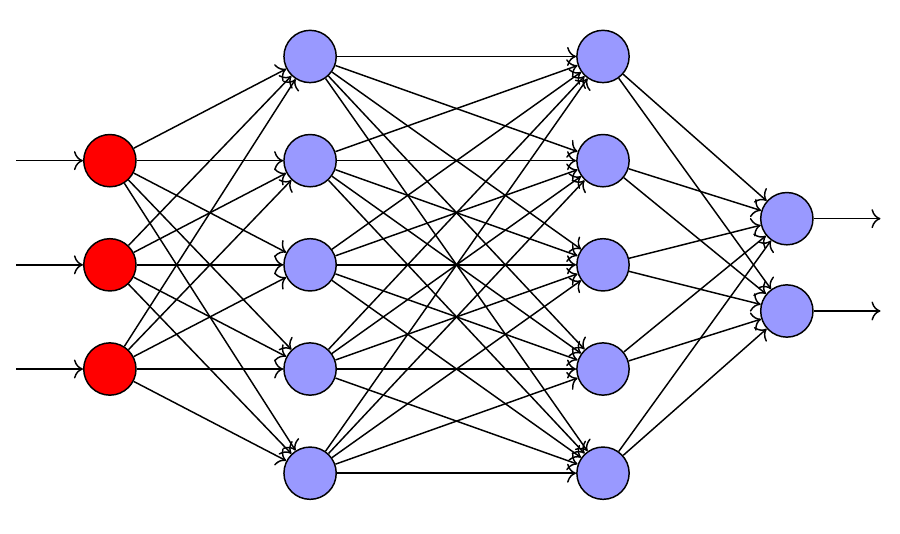
\includegraphics[width=5cm]{../images/fnn.png}
	\end{figure}
	\lstinline| modules = [] |\\
	\lstinline| modules.append(nn.Linear(3, 5)) |\\
	\lstinline| modules.append(nn.ReLU()) |\\
	\lstinline| modules.append(nn.Linear(5, 5)) |\\
	\lstinline| modules.append(nn.ReLU()) |\\
	\lstinline| modules.append(nn.Linear(5, 2)) |\\
	\lstinline| model = nn.Sequential(*modules) |
}

\end{document}